\documentclass{report}
\usepackage[spanish]{babel}
\usepackage[left=2.5cm, right=2.5cm, top=3cm, bottom=3cm]{geometry}
\usepackage{enumerate}
\usepackage{graphicx}
\usepackage{booktabs}
\usepackage{tabularx}
\usepackage{enumitem}
\usepackage{amsmath}
\usepackage{amsfonts}
\usepackage{float}
\usepackage{hyperref}

\setlength{\parindent}{0pt}

\begin{document}

    \begin{titlepage}
        \centering
        {\bfseries\Huge Manual de Usuario \par}
        \vspace*{1cm}
        \vspace*{3cm}
        \vspace*{1cm}
        {\LARGE \textbf{Nombre: Gestión de campeonatos de béisbol} }
        \vfill
        {\bfseries\LARGE Autores: \par}
        {\Large Ariadna Vel\'azquez Rey  C311 \par}
        {\Large L\'ia L\'opez Rosales  C312 \par}
        {\Large Carlos Daniel Largacha Leal  C312 \par}
        {\Large Gabriel Andr\'es Pla Lasa  C311 \par}
        {\Large Raidel Miguel Cabellud Lizaso C311 \par}
        \vfill
    \end{titlepage}

    \section*{Objetivo del proyecto}
    La \textbf{Liga Nacional de Béisbol (LNB PRO)} es la plataforma oficial de gestión deportiva de la
    liga: permite consultar y analizar la información relevante de las series, los equipos y los peloteros,
    proporcionando herramientas de gestión táctica (alineaciones, cambios y reportes oficiales) que soportan
    la toma de decisiones basada en estadísticas detalladas y actualizadas. El sistema es accesible desde
    cualquier navegador y se adapta a distintos perfiles: administradores, directores técnicos, usuarios
    generales e invitados.

    \section*{Requerimientos Técnicos}
    \begin{itemize}
        \item Dispositivos capaces de ejecutar navegadores modernos con conexión a internet estable.
        \item En caso de ejecutar una versión local también se necesitan Node.js (18+), Python (3.10+) y
        PostgreSQL,
        con al menos 1~GB de espacio disponible.
    \end{itemize}

    \section*{Forma de instalar la aplicación (modo local)}
    \begin{enumerate}
        \item Crear una base de datos en PostgreSQL y configurar los datos de conexión
        (\texttt{DB\_NAME}, \texttt{DB\_USER}, \texttt{DB\_PASSWORD}, \texttt{DB\_HOST}, \texttt{DB\_PORT})
        en el archivo \texttt{.env} de la carpeta principal.
        \item Instalar las dependencias del backend con los paquetes de \texttt{pyproject.toml}
        (activar el entorno virtual con \texttt{source python\_enviroment/bin/activate}).
        \item Ejecutar las migraciones:
        \texttt{python manage.py makemigrations} y \texttt{python manage.py migrate}.
        \item (Opcional) Sembrar la base de datos con datos de demostración:
        \texttt{python populate\_db.py}. Esto crea equipos, series simuladas, jugadores y los usuarios
        de prueba.
        \item Instalar los módulos de React con \texttt{npm install} desde la carpeta
        \texttt{Baseball\_Management}.
        \item Arrancar la aplicación con el comando \texttt{npm start} desde \texttt{Baseball\_Management}
        (levanta simultáneamente el frontend en \texttt{http://localhost:3000} y el backend en
        \texttt{http://127.0.0.1:8000}).
    \end{enumerate}

    \section*{Cuentas de demostración}
    El sembrador (\texttt{populate\_db.py}) crea tres cuentas de prueba que permiten probar todos los
    roles del sistema:

    \begin{center}
    \begin{tabular}{lll}
        \toprule
        \textbf{Correo} & \textbf{Contraseña} & \textbf{Rol} \\
        \midrule
        \texttt{lialopez@gmail.com} & \texttt{lia} & Admin \\
        \texttt{director@test.com} & \texttt{director} & Director Técnico \\
        \texttt{general@test.com} & \texttt{general} & Usuario General \\
        \bottomrule
    \end{tabular}
    \end{center}

    Además, cualquier visitante puede acceder como \textbf{invitado} (sin sesión) a toda la información
    pública, o registrarse por su cuenta para usar los servicios personalizados.

    \section*{Acceso al sistema}
    Al entrar en la aplicación se muestra la \textbf{Landing pública} con las estadísticas del campeonato
    (ver Figura~\ref{fig:landing}). Desde la cabecera se puede iniciar sesión o crear una cuenta.

    \begin{figure}[H]
        \centering
        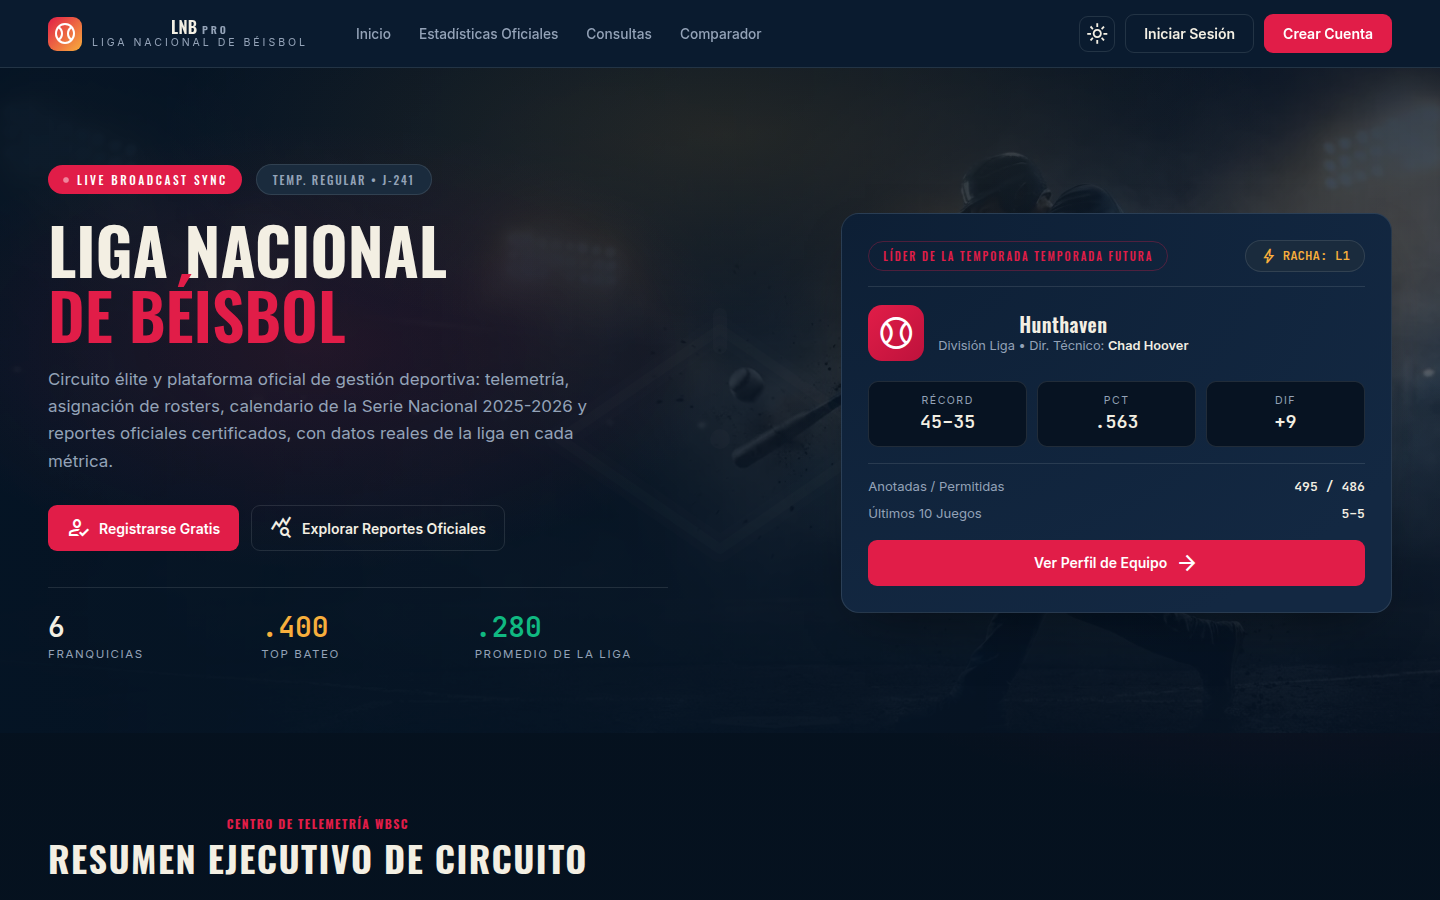
\includegraphics[width=0.62\textwidth]{img/img_1.png}
        \caption{Landing pública de la Liga Nacional de Béisbol}
        \label{fig:landing}
    \end{figure}

    \subsection*{Inicio de Sesión}
    Para acceder, el usuario debe abrir el modal de inicio de sesión desde la cabecera (botón
    \texttt{Iniciar Sesión}) e introducir su correo y contraseña. Según el rol autenticado se mostrarán
    las funcionalidades a las que tiene acceso.

    \begin{figure}[H]
        \centering
        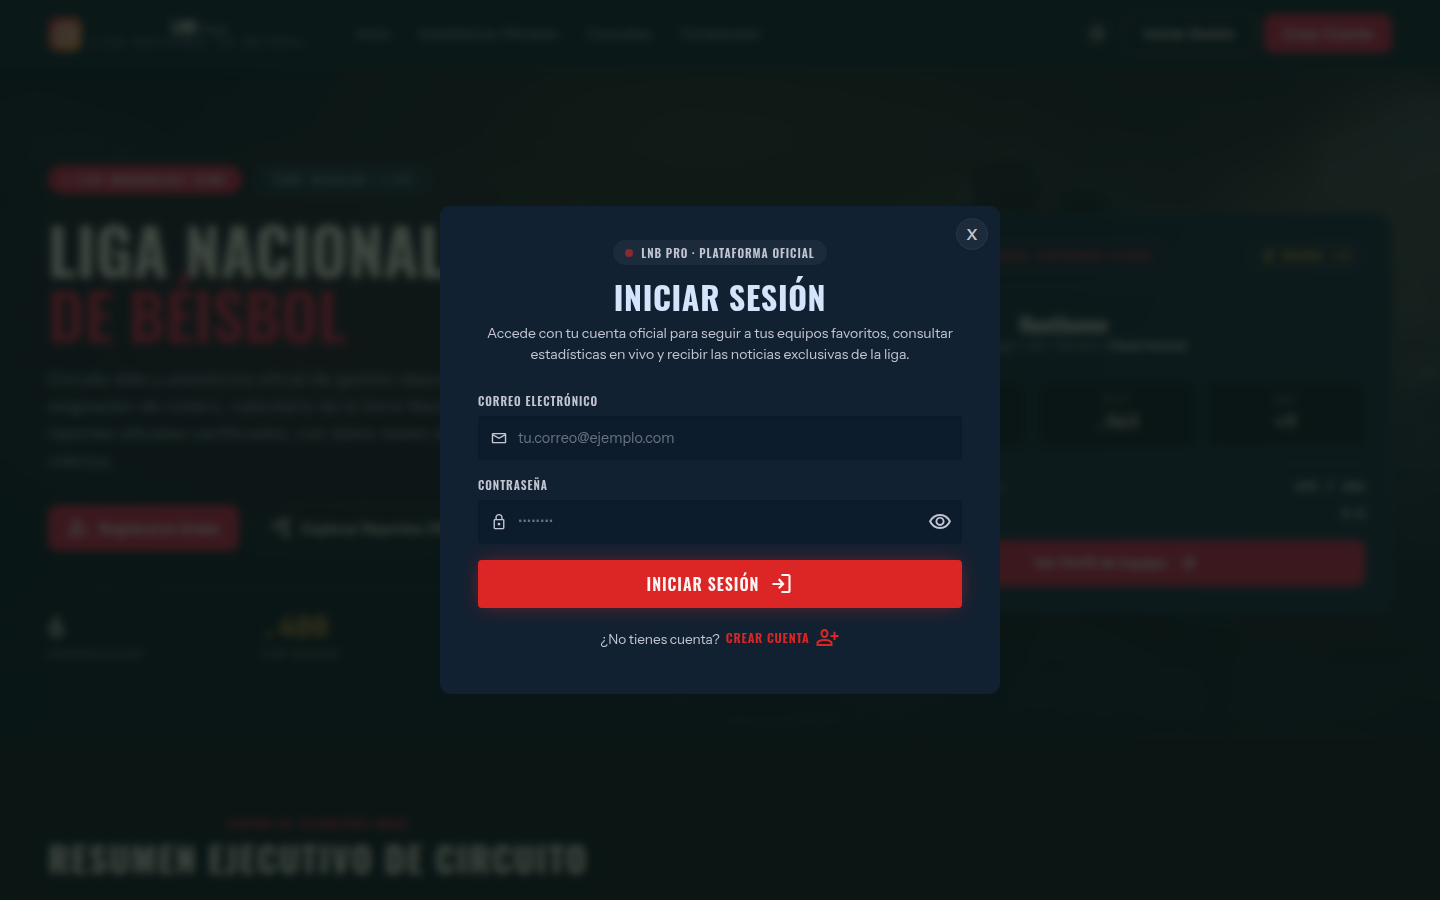
\includegraphics[width=0.62\textwidth]{img/img_2.png}
        \caption{Modal de inicio de sesión}
    \end{figure}

    \subsection*{Registro público}
    Un visitante puede crear una cuenta en el botón \texttt{Crear Cuenta}. El formulario solicita nombre,
    apellido, correo y contraseña; al registrarse se crea automáticamente un usuario con rol
    \texttt{Usuario General} y se inicia la sesión.

    \begin{figure}[H]
        \centering
        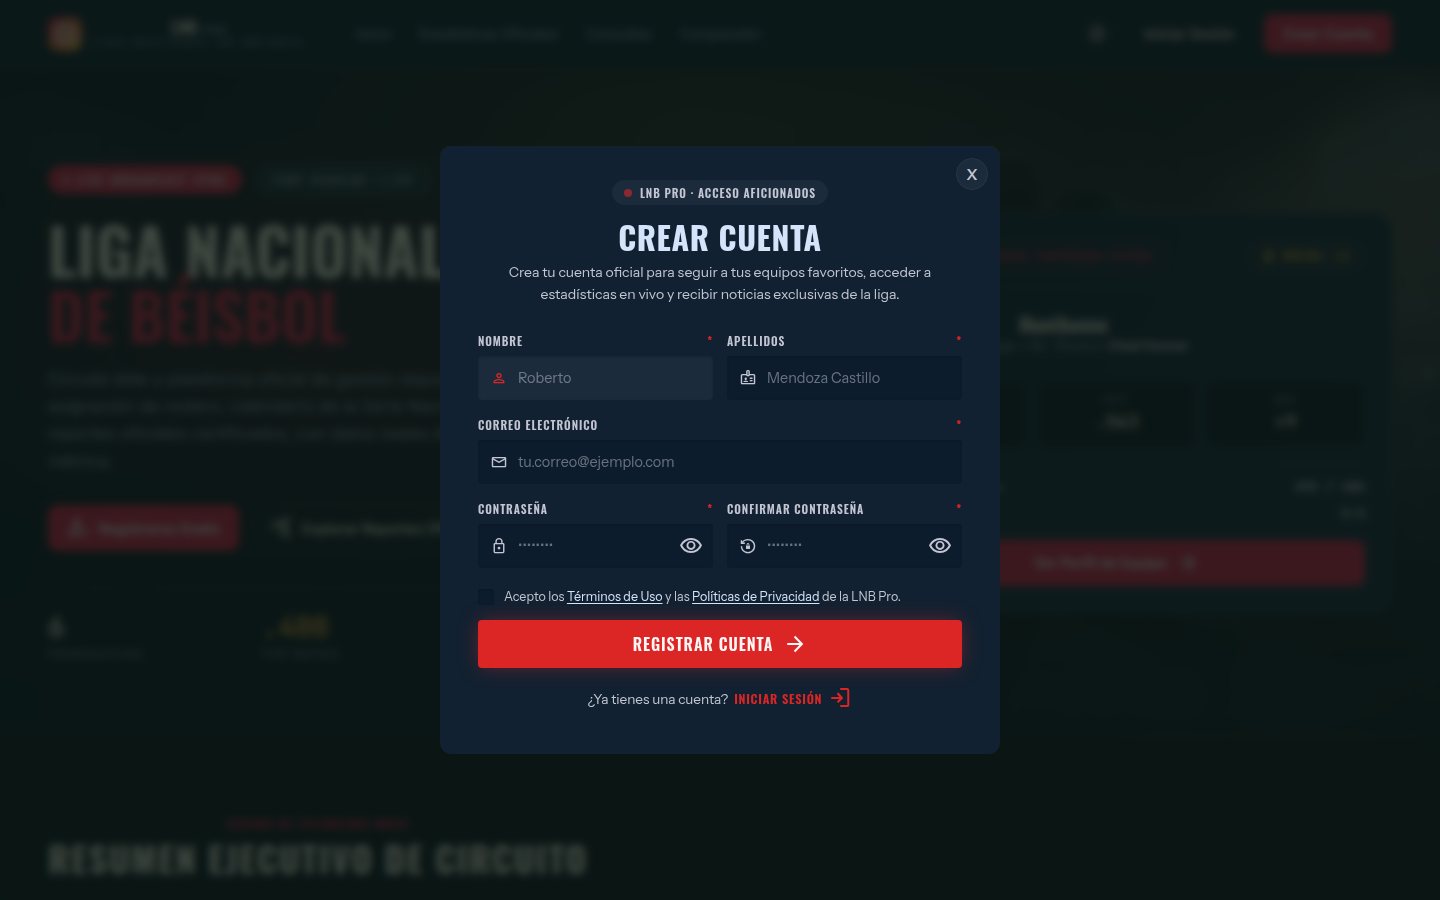
\includegraphics[width=0.62\textwidth]{img/img_3.png}
        \caption{Modal de creación de cuenta (registro público)}
    \end{figure}

    \section*{Roles del sistema}
    La aplicación diferencia cuatro perfiles:
    \begin{itemize}
        \item \textbf{Invitado:} no inicia sesión; navega toda la información pública (landing, consultas,
        reportes, perfiles) y ve los comparadores.
        \item \textbf{Usuario General:} además de lo público, dispone de ``Tu panel'', favoritos de
        equipos y jugadores, notificaciones y acceso al comparador con su cuenta.
        \item \textbf{Director Técnico:} gestiona las alineaciones y los cambios de su equipo en el
        Portal de Cambios, y consulta su historial.
        \item \textbf{Admin:} accede al Panel Administrativo con CRUD completo de todas las entidades del
        sistema.
    \end{itemize}

    \section*{Breve explicación de cada una de las opciones del sistema}

    \subsection*{Landing pública}
    La página de inicio resume el estado del campeonato: líder de la temporada, tabla de posiciones,
    líderes de bateo, jugadores estrella por posición y el palmarés de campeones de las últimas temporadas.
    Todos los elementos enlazan con sus perfiles o reportes correspondientes.

    \subsection*{Tu panel y Tus favoritos (Usuario General)}
    Con la sesión iniciada, la landing incorpora la sección \texttt{Tu panel}, que muestra la posición
    actual del equipo favorito, sus últimos juegos, la estrella del equipo con un radar compacto y el
    aviso de notificaciones. Junto a él aparece \texttt{Tus favoritos}, con los equipos y jugadores que
    el usuario sigue; cada tarjeta enlaza con el perfil correspondiente.

    \begin{figure}[H]
        \centering
        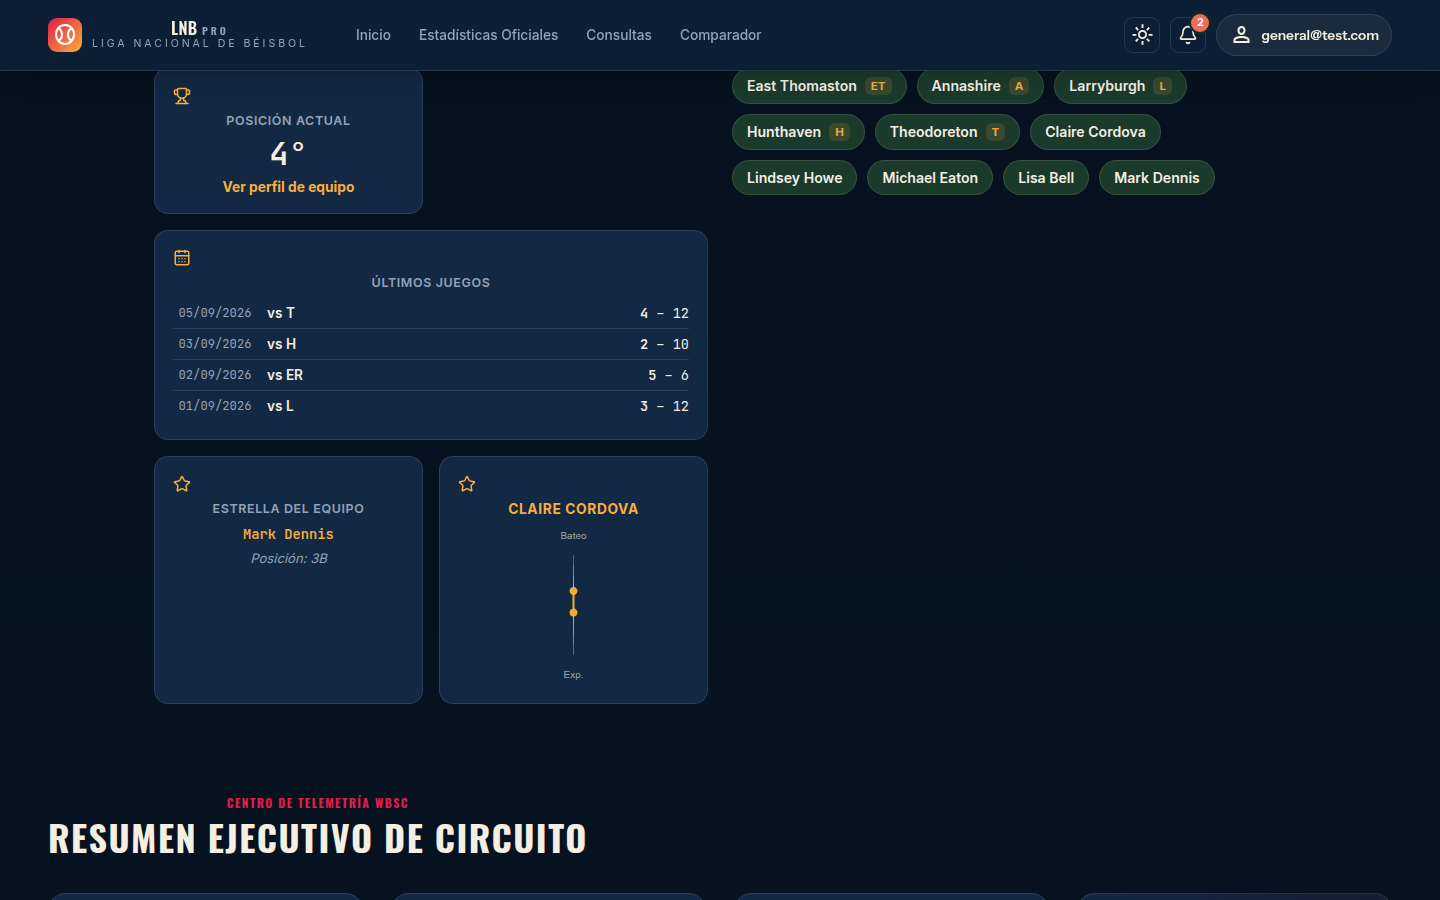
\includegraphics[width=0.62\textwidth]{img/img_4.png}
        \caption{Secciones ``Tu panel'' y ``Tus favoritos'' para un usuario con sesión iniciada}
    \end{figure}

    \subsection*{Notificaciones}
    La campana de la cabecera muestra un contador de notificaciones no leídas. Su dropdown lista los avisos
    (por ejemplo, resultados recientes del equipo seguido), permite marcar cada una como leída y enlaza
    con el perfil del equipo o jugador relacionado. La campana consulta las notificaciones automáticamente
    cada 30 segundos.

    \begin{figure}[H]
        \centering
        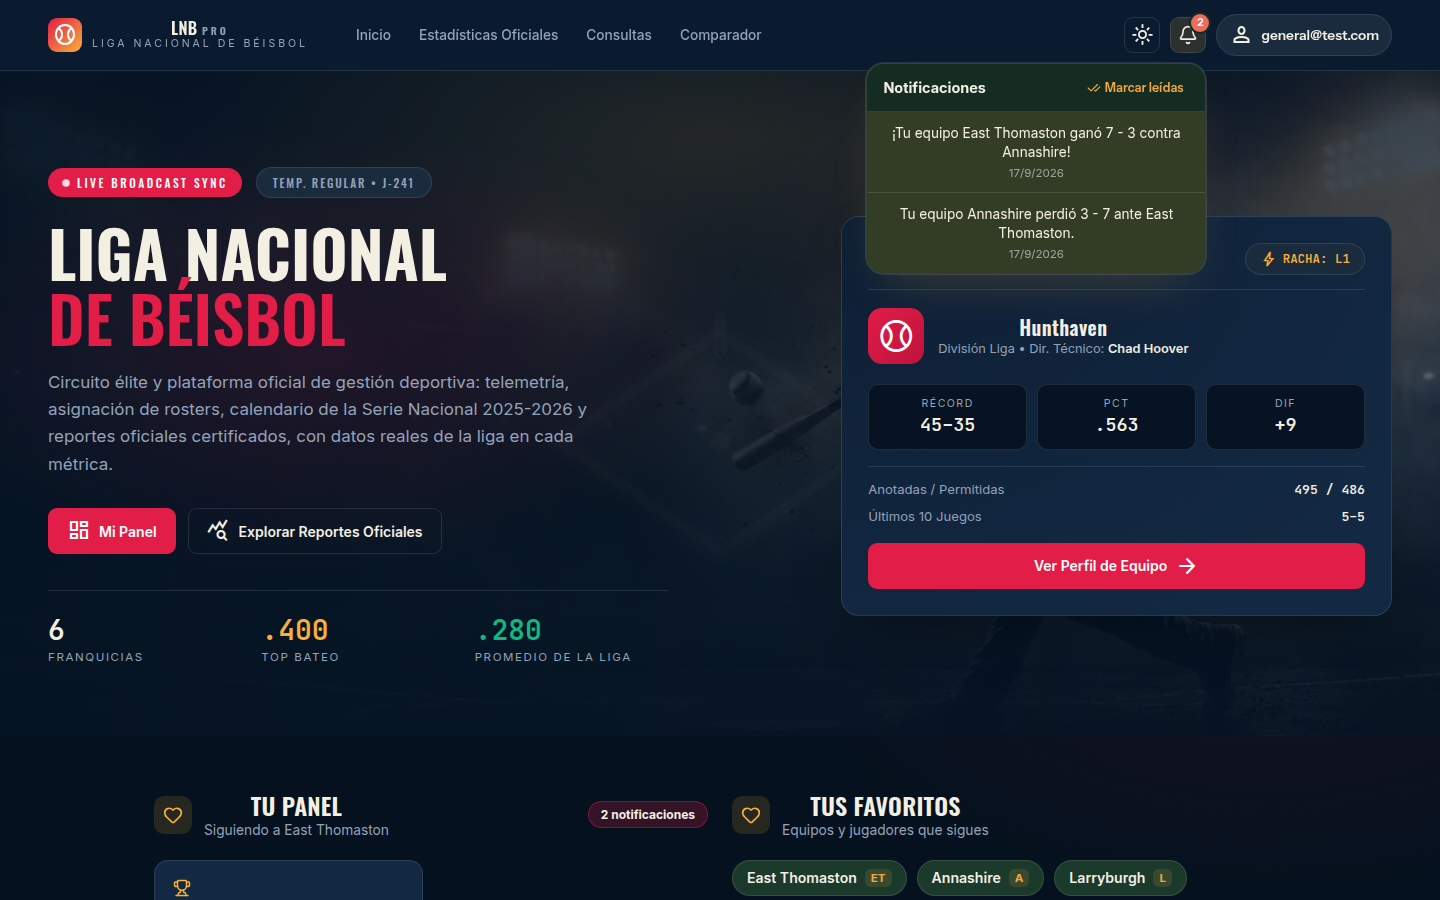
\includegraphics[width=0.62\textwidth]{img/img_5.png}
        \caption{Dropdown de notificaciones con avisos de resultados del equipo seguido}
    \end{figure}

    \subsection*{Panel de cambios (Director Técnico)}
    El Portal de Cambios (\texttt{/dt/cambios}) permite al director técnico de un equipo:
    \begin{itemize}
        \item Seleccionar un \textbf{juego pendiente} de su calendario y ver la \textbf{previa del
        encuentro} con la efectividad media del rival.
        \item Disfrutar de la \textbf{Lineup Titular WBSC} (regla regulatoria mostrada en la interfaz) con
        los promedios reales de cada jugador.
        \item Visualizar la \textbf{posición defensiva en el campo} (diamante con los 9 chips
        posicionales: Pitcher, Catcher, 1B, 2B, 3B, SS, LF, CF, RF).
        \item Ejecutar \textbf{sustituciones} desde el bullpen y la reserva activa, filtrando jugadores por
        posición.
        \item Consultar las \textbf{métricas} del equipo: efectividad media, posiciones en fila, jugadores
        en reserva y cambios registrados.
    \end{itemize}
    Solo se ofrecen juegos futuros; el sistema valida en el backend que no se pueda registrar un cambio en
    un juego ya disputado.

    \begin{figure}[H]
        \centering
        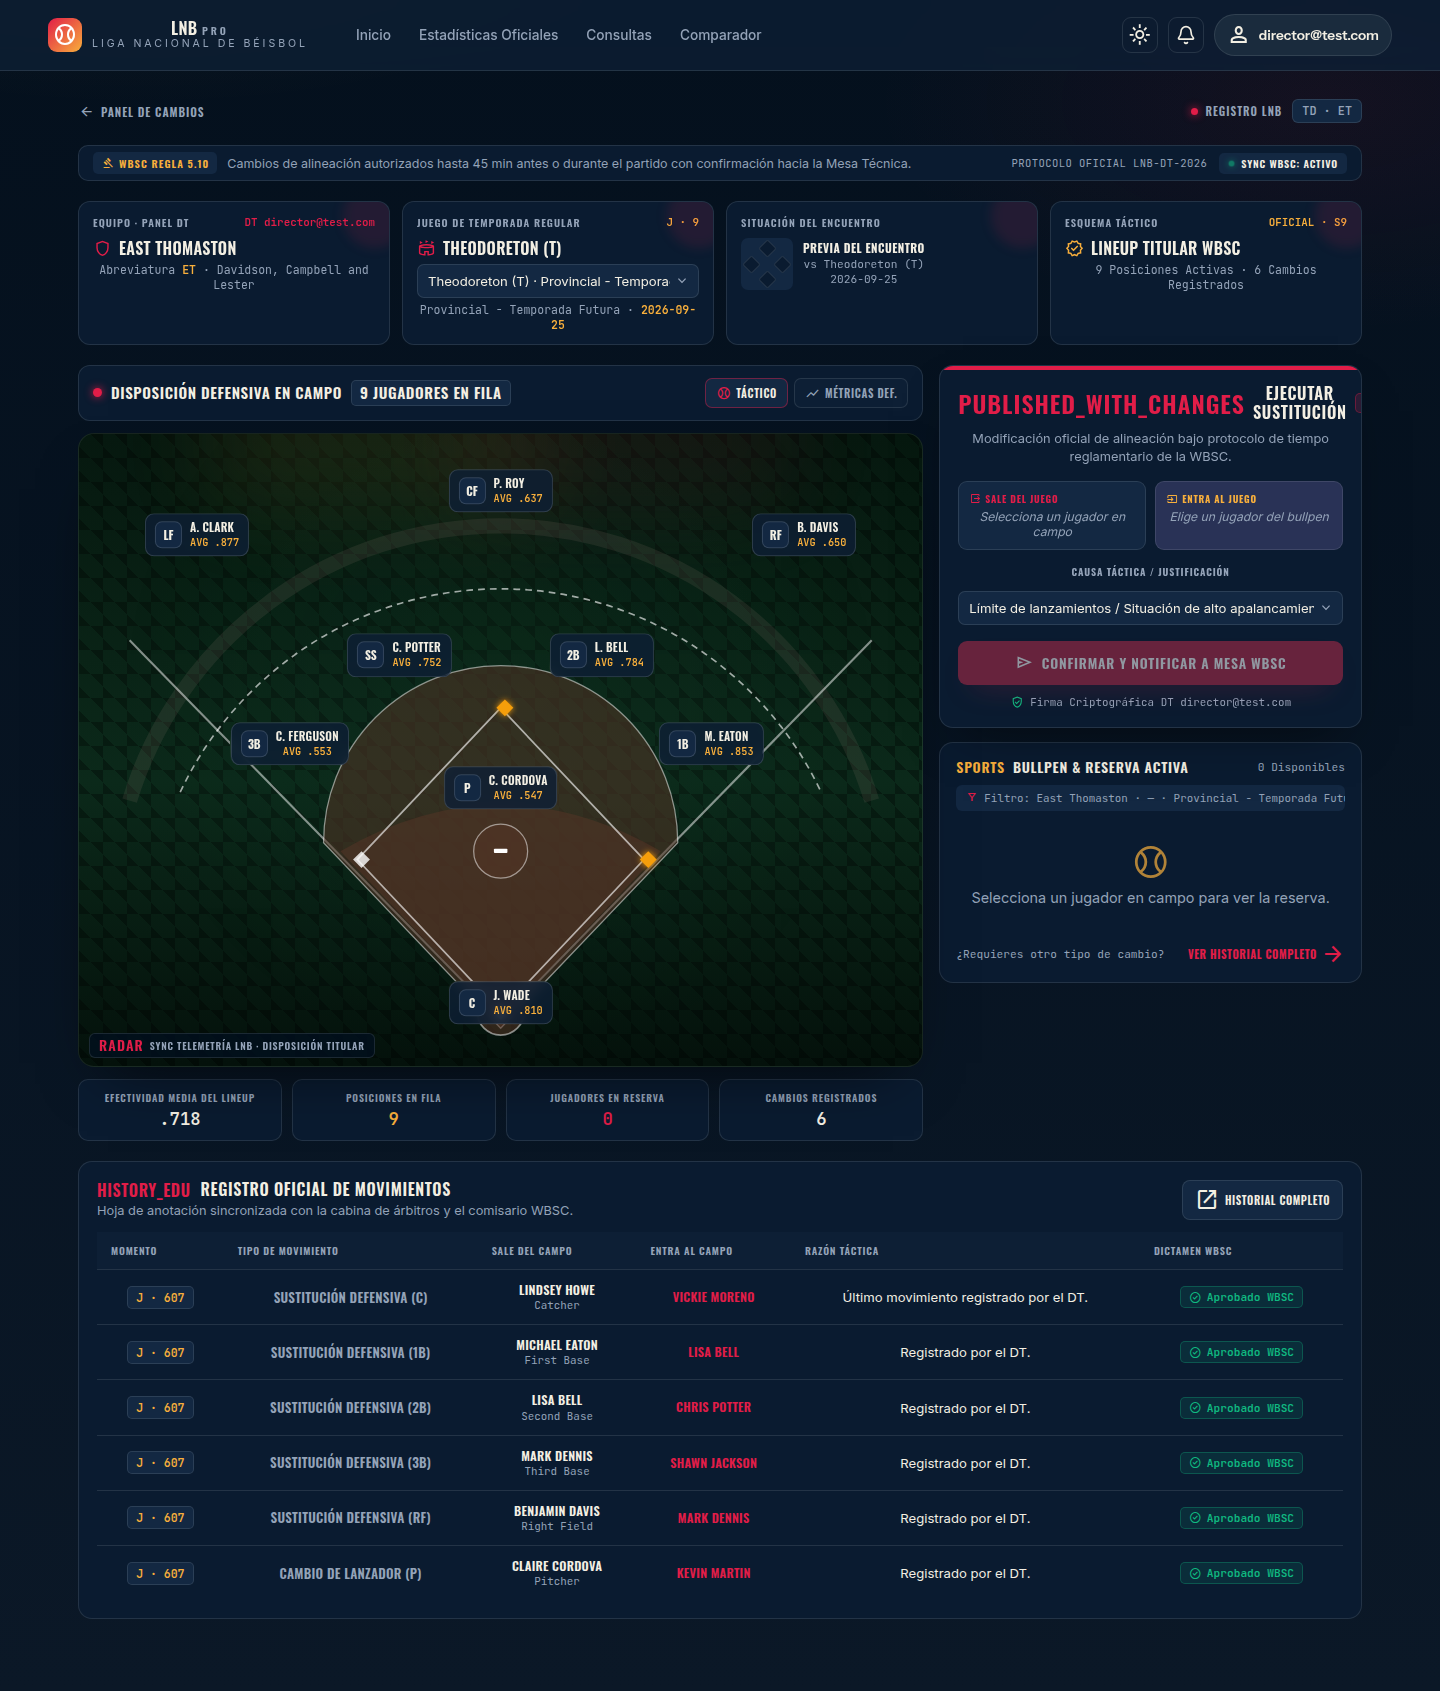
\includegraphics[width=0.7\textwidth]{img/img_6.png}
        \caption{Panel de cambios del Director Técnico con el lineup titular y el diamante defensivo}
    \end{figure}

    \subsection*{Historial de cambios (Director Técnico)}
    La página \texttt{/dt/listar-cambios} presenta el historial completo de sustituciones del equipo en una
    tabla ordenable y con paginación, con el detalle de jugador que sale, jugador que entra, posición,
    fecha y el juego asociado. Desde aquí se puede registrar un nuevo cambio o eliminar uno existente.

    \begin{figure}[H]
        \centering
        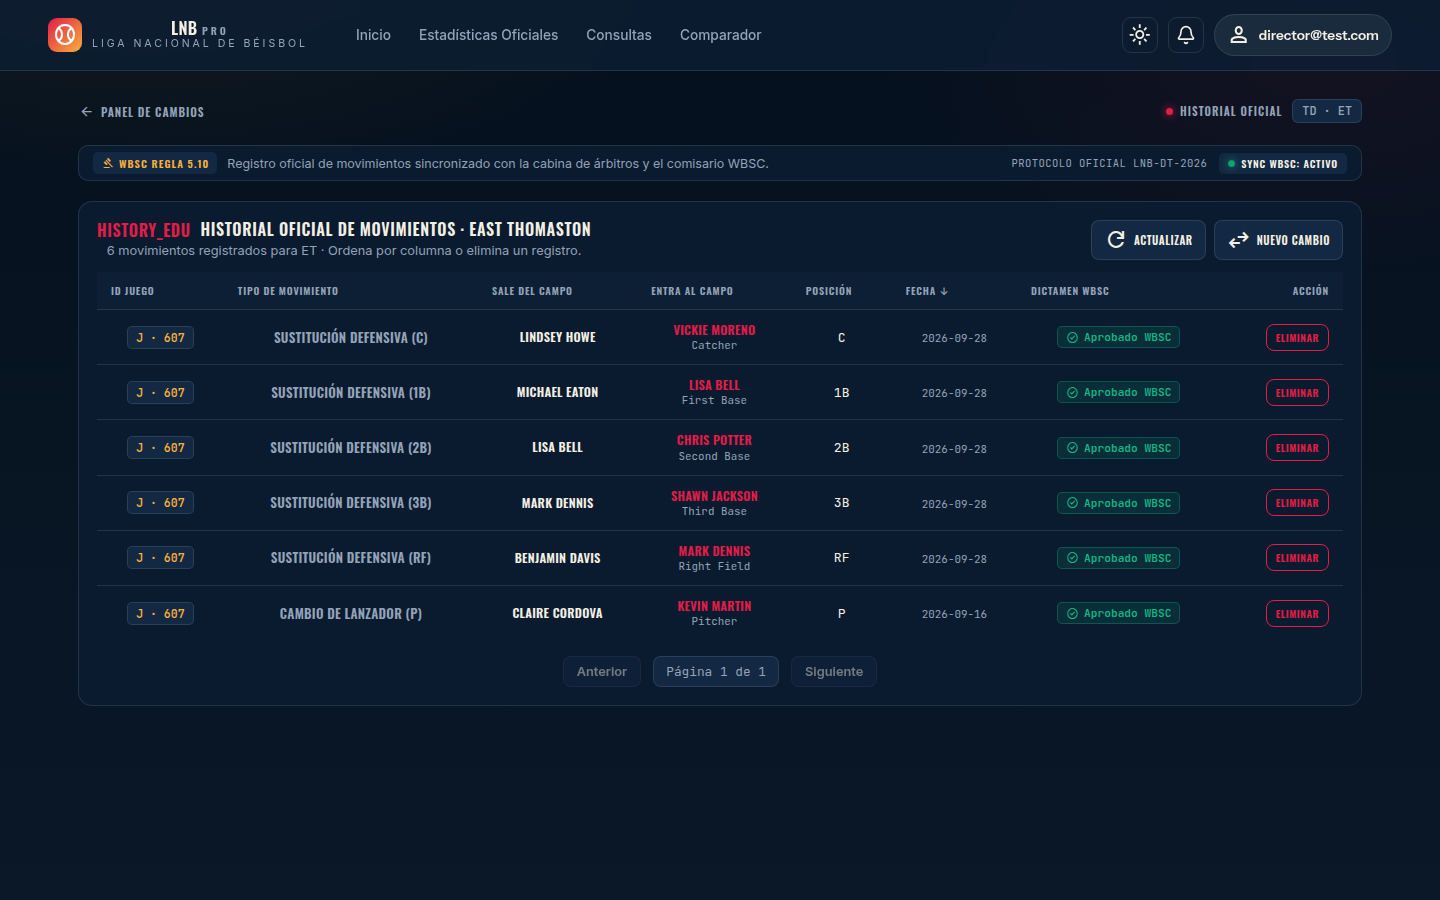
\includegraphics[width=0.62\textwidth]{img/img_7.png}
        \caption{Historial de cambios técnicos del equipo}
    \end{figure}

    \subsection*{Panel administrativo (Admin)}
    El Admin accede al \texttt{Panel Administrativo} (\texttt{/admin/{tabla}}), que agrupa formularios y
    CRUD de 20 entidades: personas, equipos, jugadores, series, temporadas, posiciones, marcadores,
    alineaciones, directores técnicos, etc. El panel permite:
    \begin{itemize}
        \item \textbf{Listar} las filas de cada tabla con sus columnas y KPIs.
        \item \textbf{Registrar} nuevas filas mediante formularios dinámicos generados por entidad.
        \item \textbf{Modificar} registros existentes.
        \item \textbf{Eliminar} registros, con confirmación.
    \end{itemize}

    \begin{figure}[H]
        \centering
        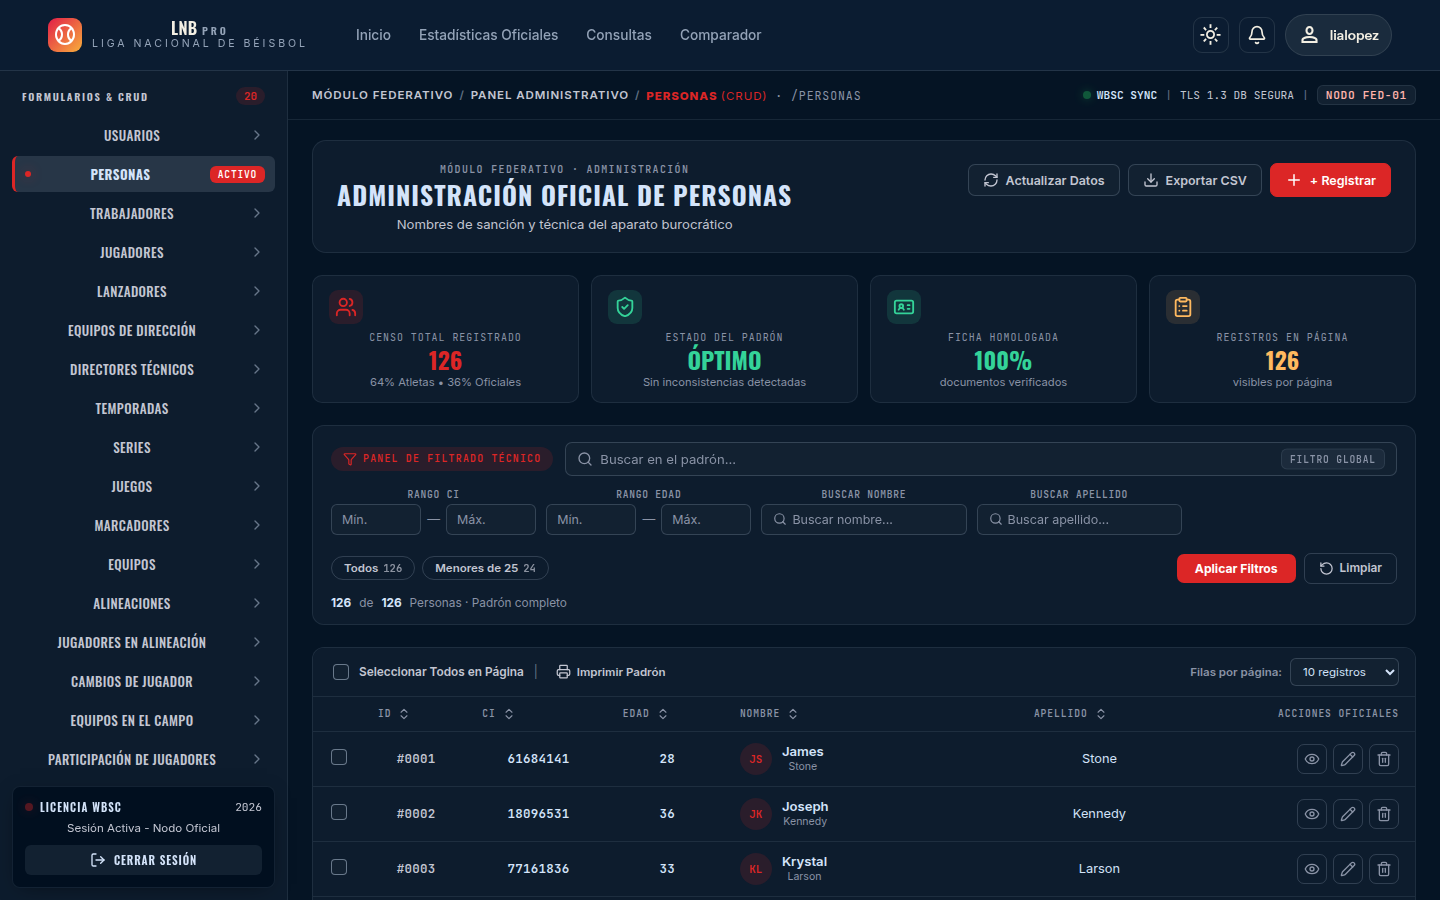
\includegraphics[width=0.62\textwidth]{img/img_8.png}
        \caption{Panel Administrativo: listado (leer) de una tabla}
    \end{figure}

    \begin{figure}[H]
        \centering
        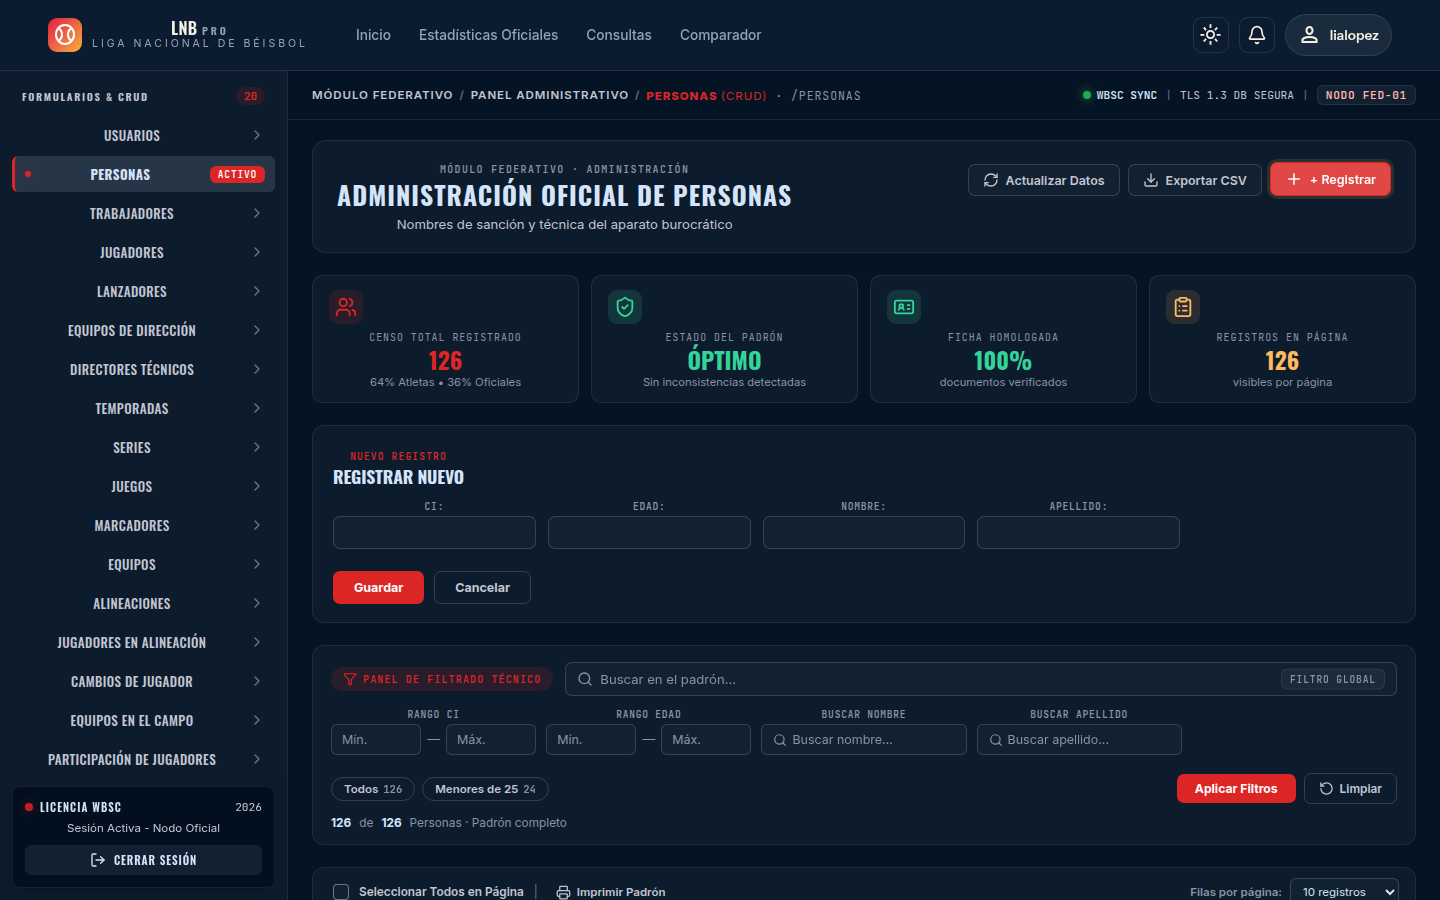
\includegraphics[width=0.62\textwidth]{img/img_9.png}
        \caption{Panel Administrativo: formulario para registrar (crear) una nueva fila}
    \end{figure}

    \subsection*{Consultas dinámicas}
    Cualquier usuario (sin importar el rol) puede consultar las tablas del sistema desde
    \texttt{Consultas} (\texttt{/consultas/{tabla}}), con listado paginado y filtros por campo según el
    tipo de dato (texto, número o fecha). Las tablas disponibles incluyen Series, Equipos, Personas,
    Jugadores, Juegos y Marcadores, entre otras.

    \begin{figure}[H]
        \centering
        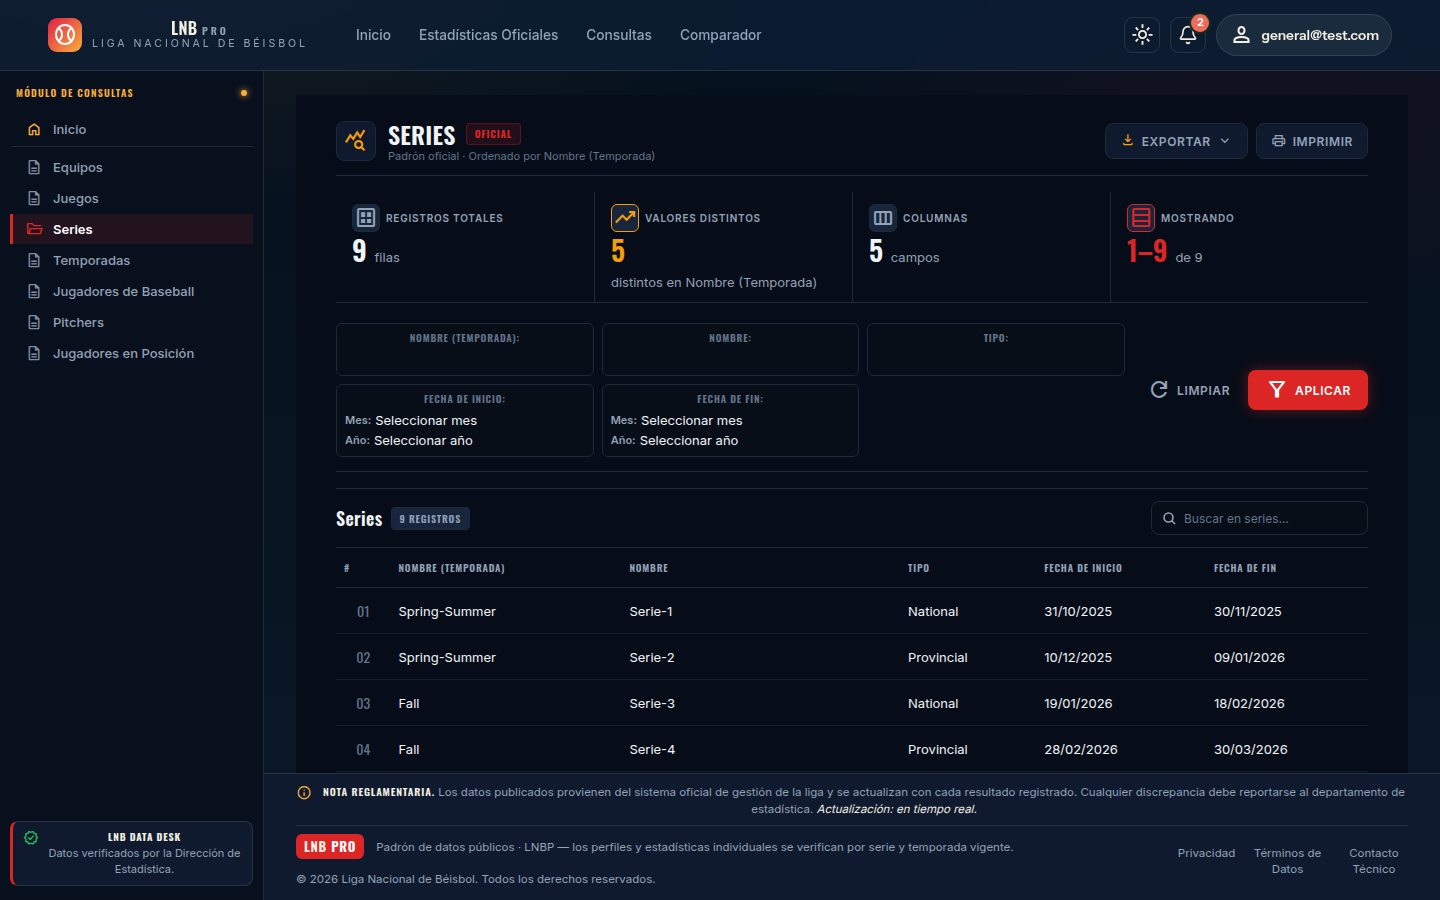
\includegraphics[width=0.62\textwidth]{img/img_10.png}
        \caption{Consulta dinámica sobre la tabla Series con filtros}
    \end{figure}

    \subsection*{Estadísticas (reportes oficiales)}
    El módulo \texttt{Estadísticas} agrupa los reportes oficiales de la liga: campeones por temporada,
    jugadores estrella, promedio de bateo, estadísticas por equipo, entre otros. Cada reporte permite
    seleccionar parámetros (temporada, serie o equipo) y se presenta en una tabla con KPIs y opciones de
    paginación. Los invitados pueden consultarlos; la exportación requiere una cuenta.

    \begin{figure}[H]
        \centering
        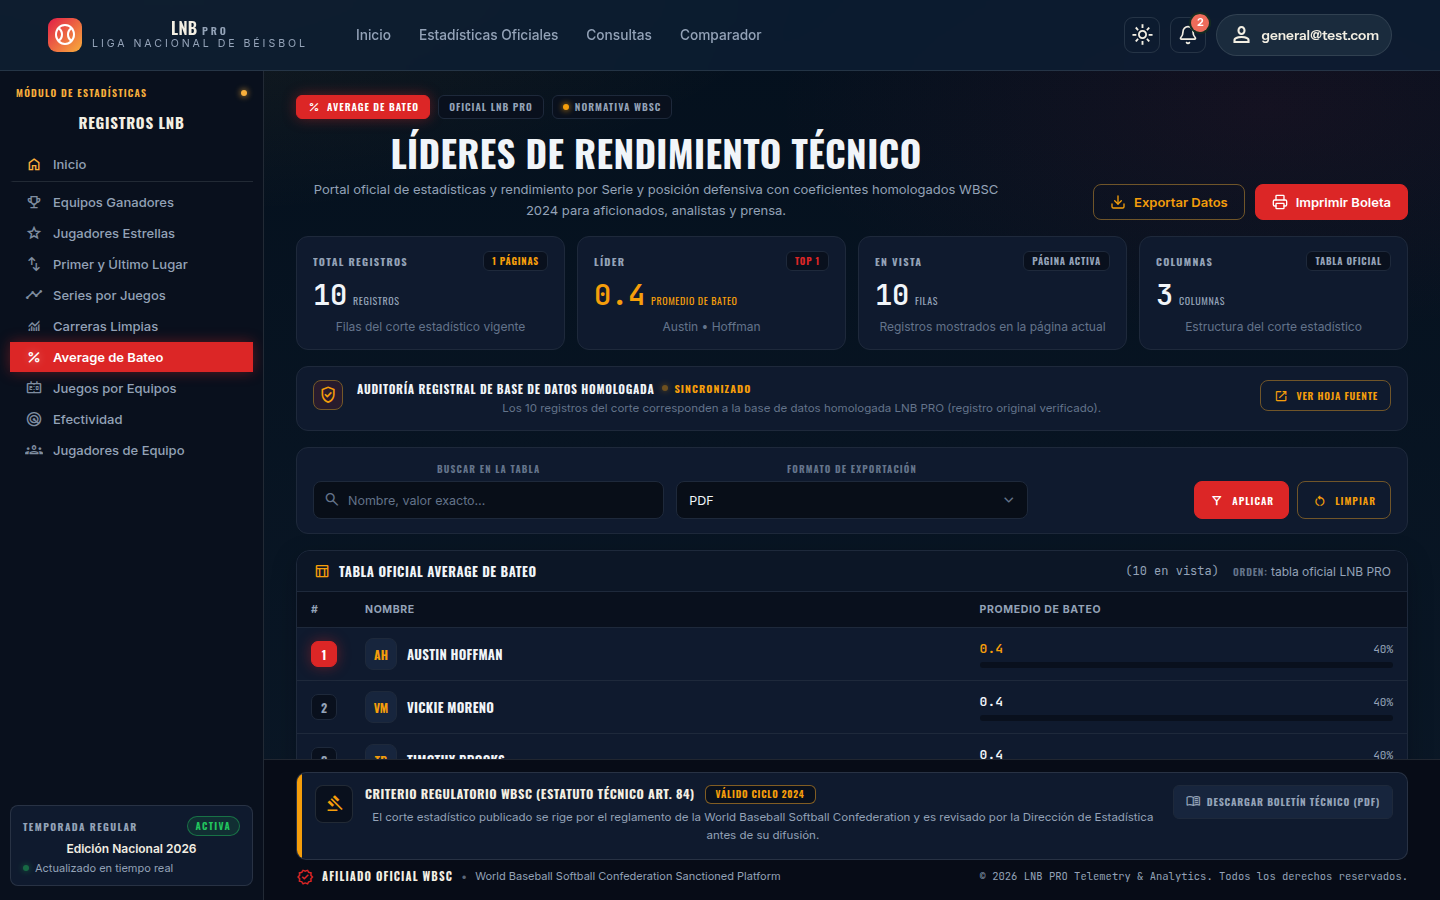
\includegraphics[width=0.62\textwidth]{img/img_11.png}
        \caption{Reporte oficial de Average de Bateo}
    \end{figure}

    \subsection*{Comparador de peloteros}
    El comparador (\texttt{/comparar}) permite seleccionar dos peloteros y confrontar sus métricas
    (posiciones, promedios, efectividad y estadísticas avanzadas) en una vista lado a lado. Solo los
    usuarios con cuenta pueden usarlo.

    \begin{figure}[H]
        \centering
        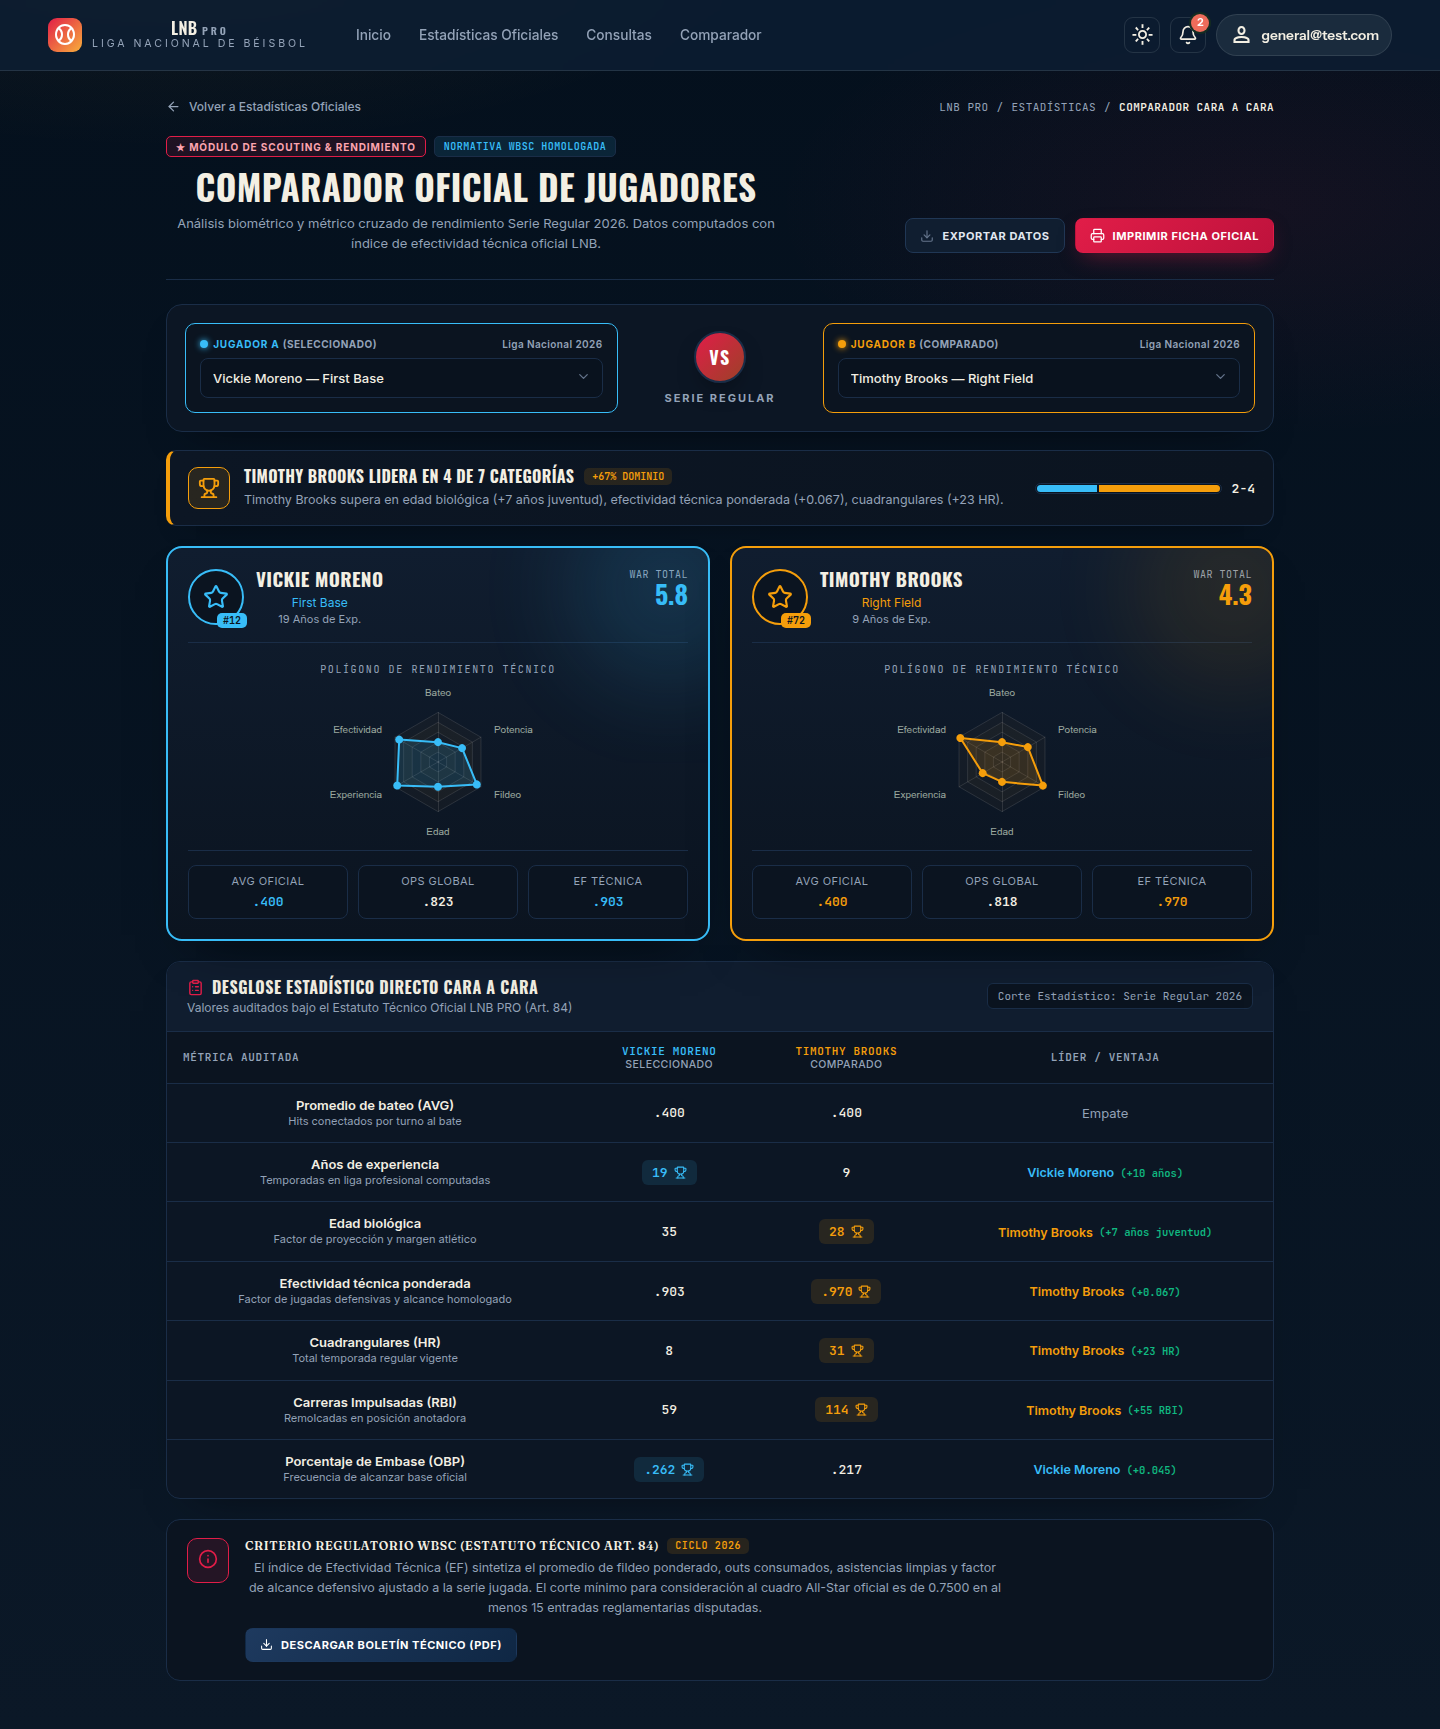
\includegraphics[width=0.7\textwidth]{img/img_12.png}
        \caption{Comparación de dos peloteros}
    \end{figure}

    \subsection*{Perfiles de equipo}
    El perfil de un equipo (\texttt{/equipo/{id}}) muestra la ficha de la franquicia (año de fundación,
    estadio, capacidad, división y eslogan), su director técnico, el récord con desglose local/visitante,
    KPIs colectivos (AVG, ERA, FLD\%), los rankings en la liga, los campeonatos obtenidos por serie, la
    distribución del plantel por grupos posicionales, los próximos juegos y el desglose de la temporada.
    Los usuarios con cuenta pueden marcar el equipo como favorito desde esta página.

    \begin{figure}[H]
        \centering
        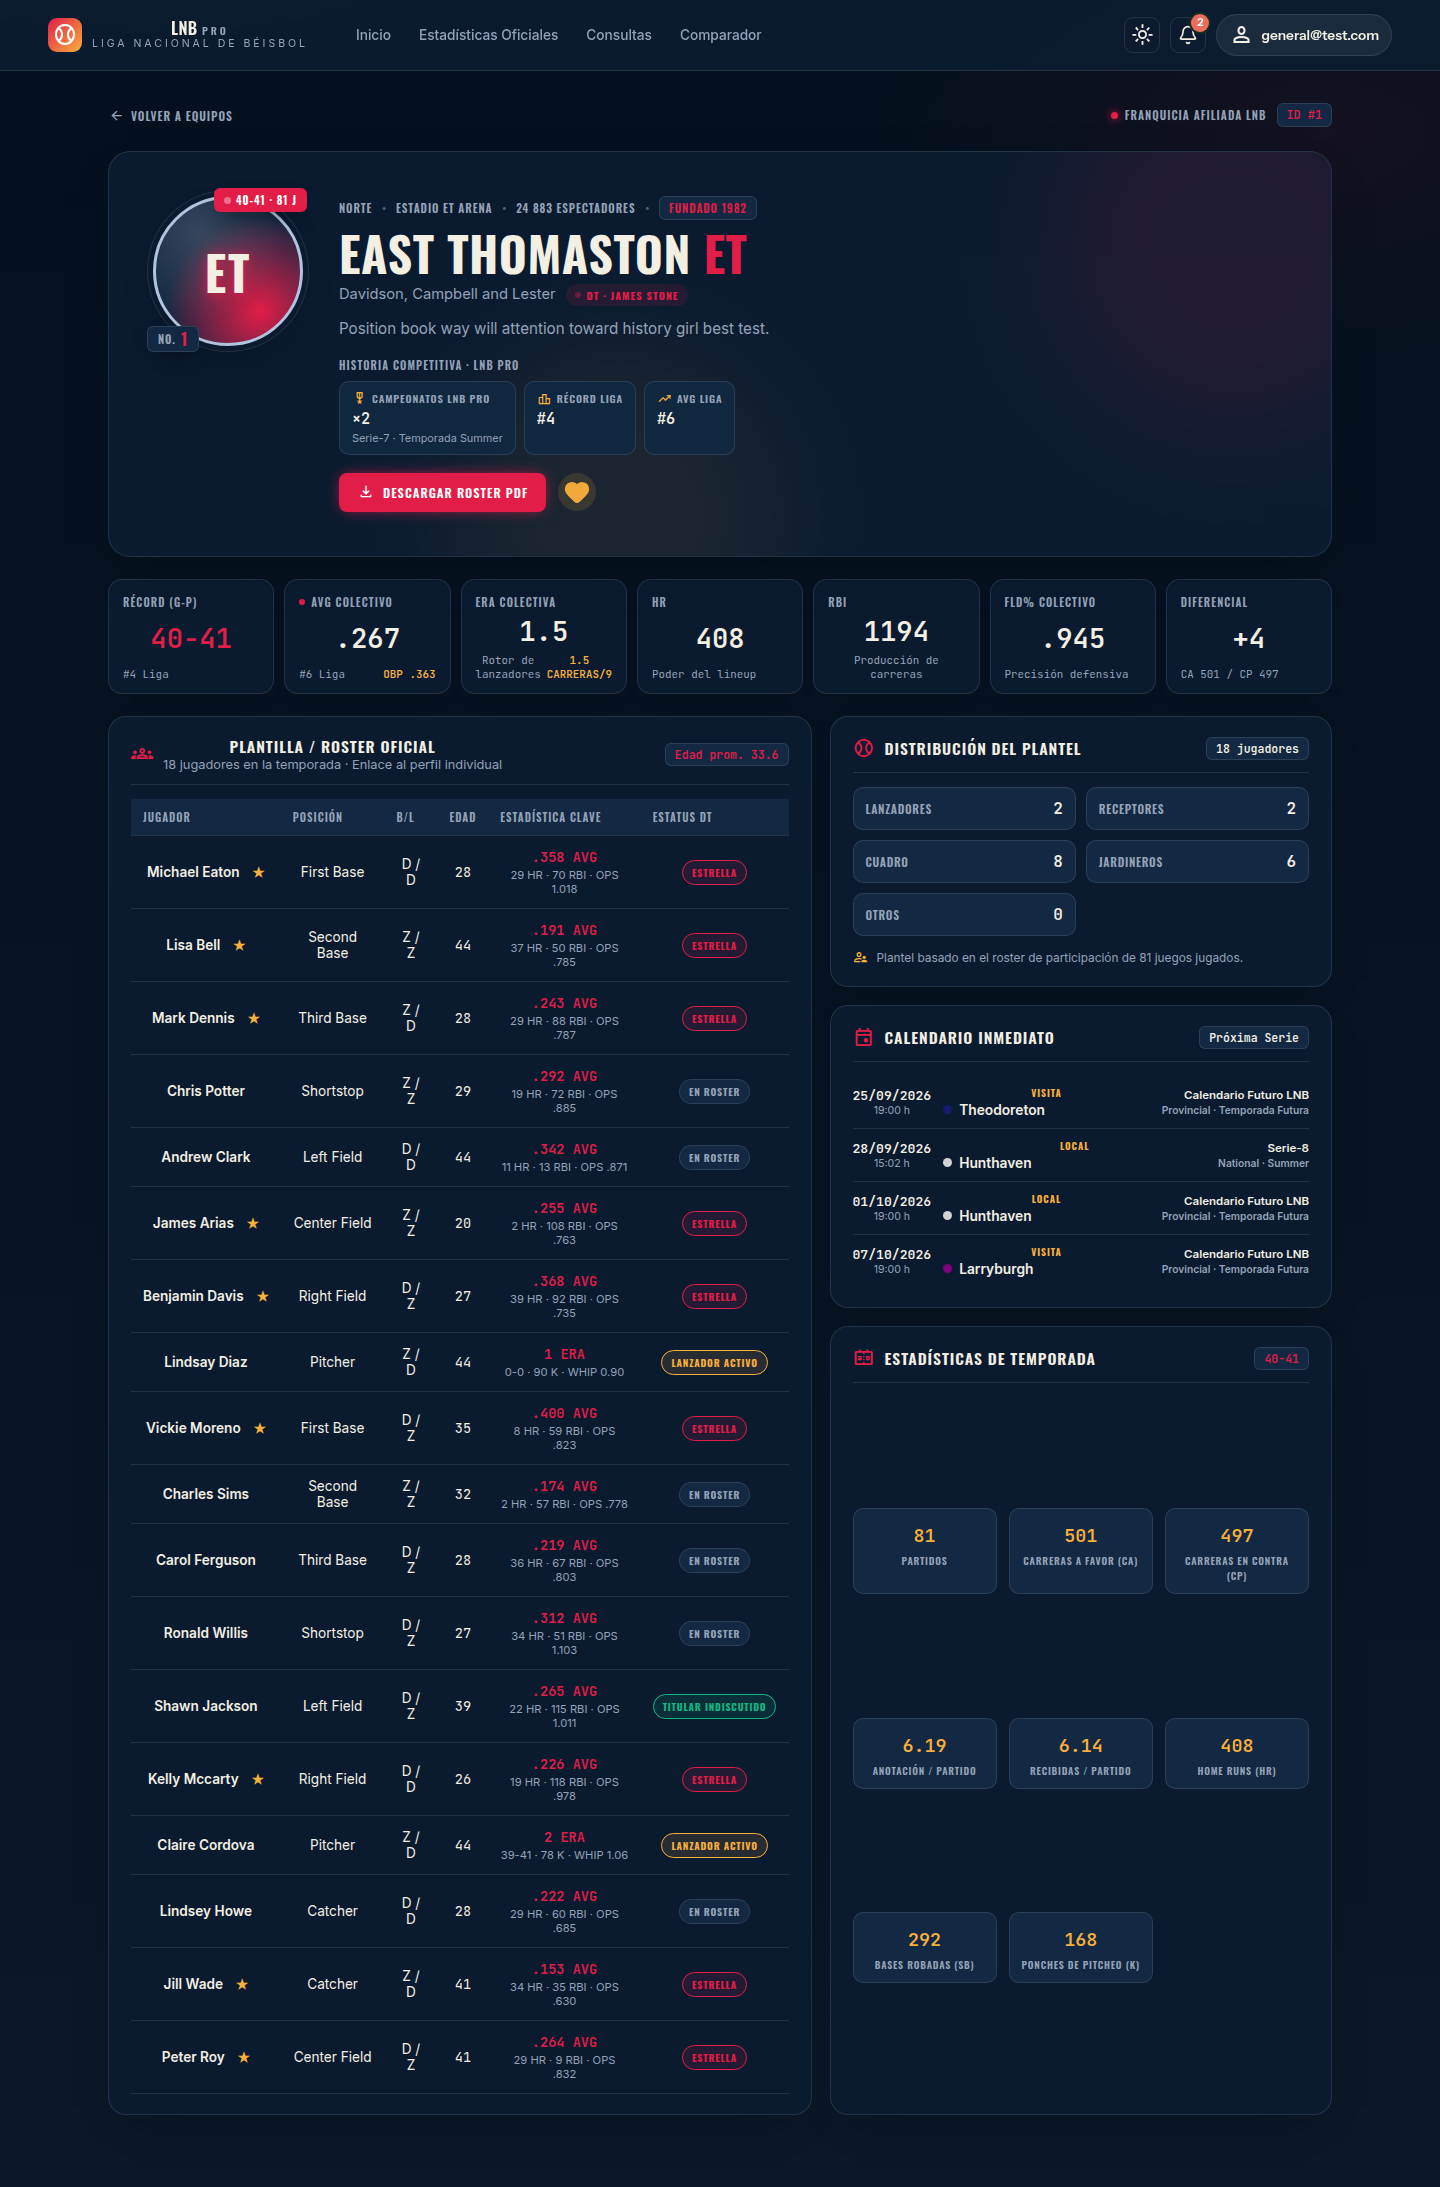
\includegraphics[width=0.7\textwidth]{img/img_13.png}
        \caption{Perfil de un equipo (ficha de franquicia, récord y plantel)}
    \end{figure}

    \subsection*{Perfiles de jugador}
    El perfil de un jugador (\texttt{/jugador/{id}}) muestra sus datos personales, sus estadísticas de
    bateo y pitcheo, y un \textbf{radar de rendimiento} (\texttt{Diamond Performance Radar}) con seis ejes
    de evaluación WBSC Statcast comparado contra la media de la liga, junto con su trayectoria reciente en
    las últimas cinco series. Los usuarios con cuenta pueden añadirlo a favoritos.

    \begin{figure}[H]
        \centering
        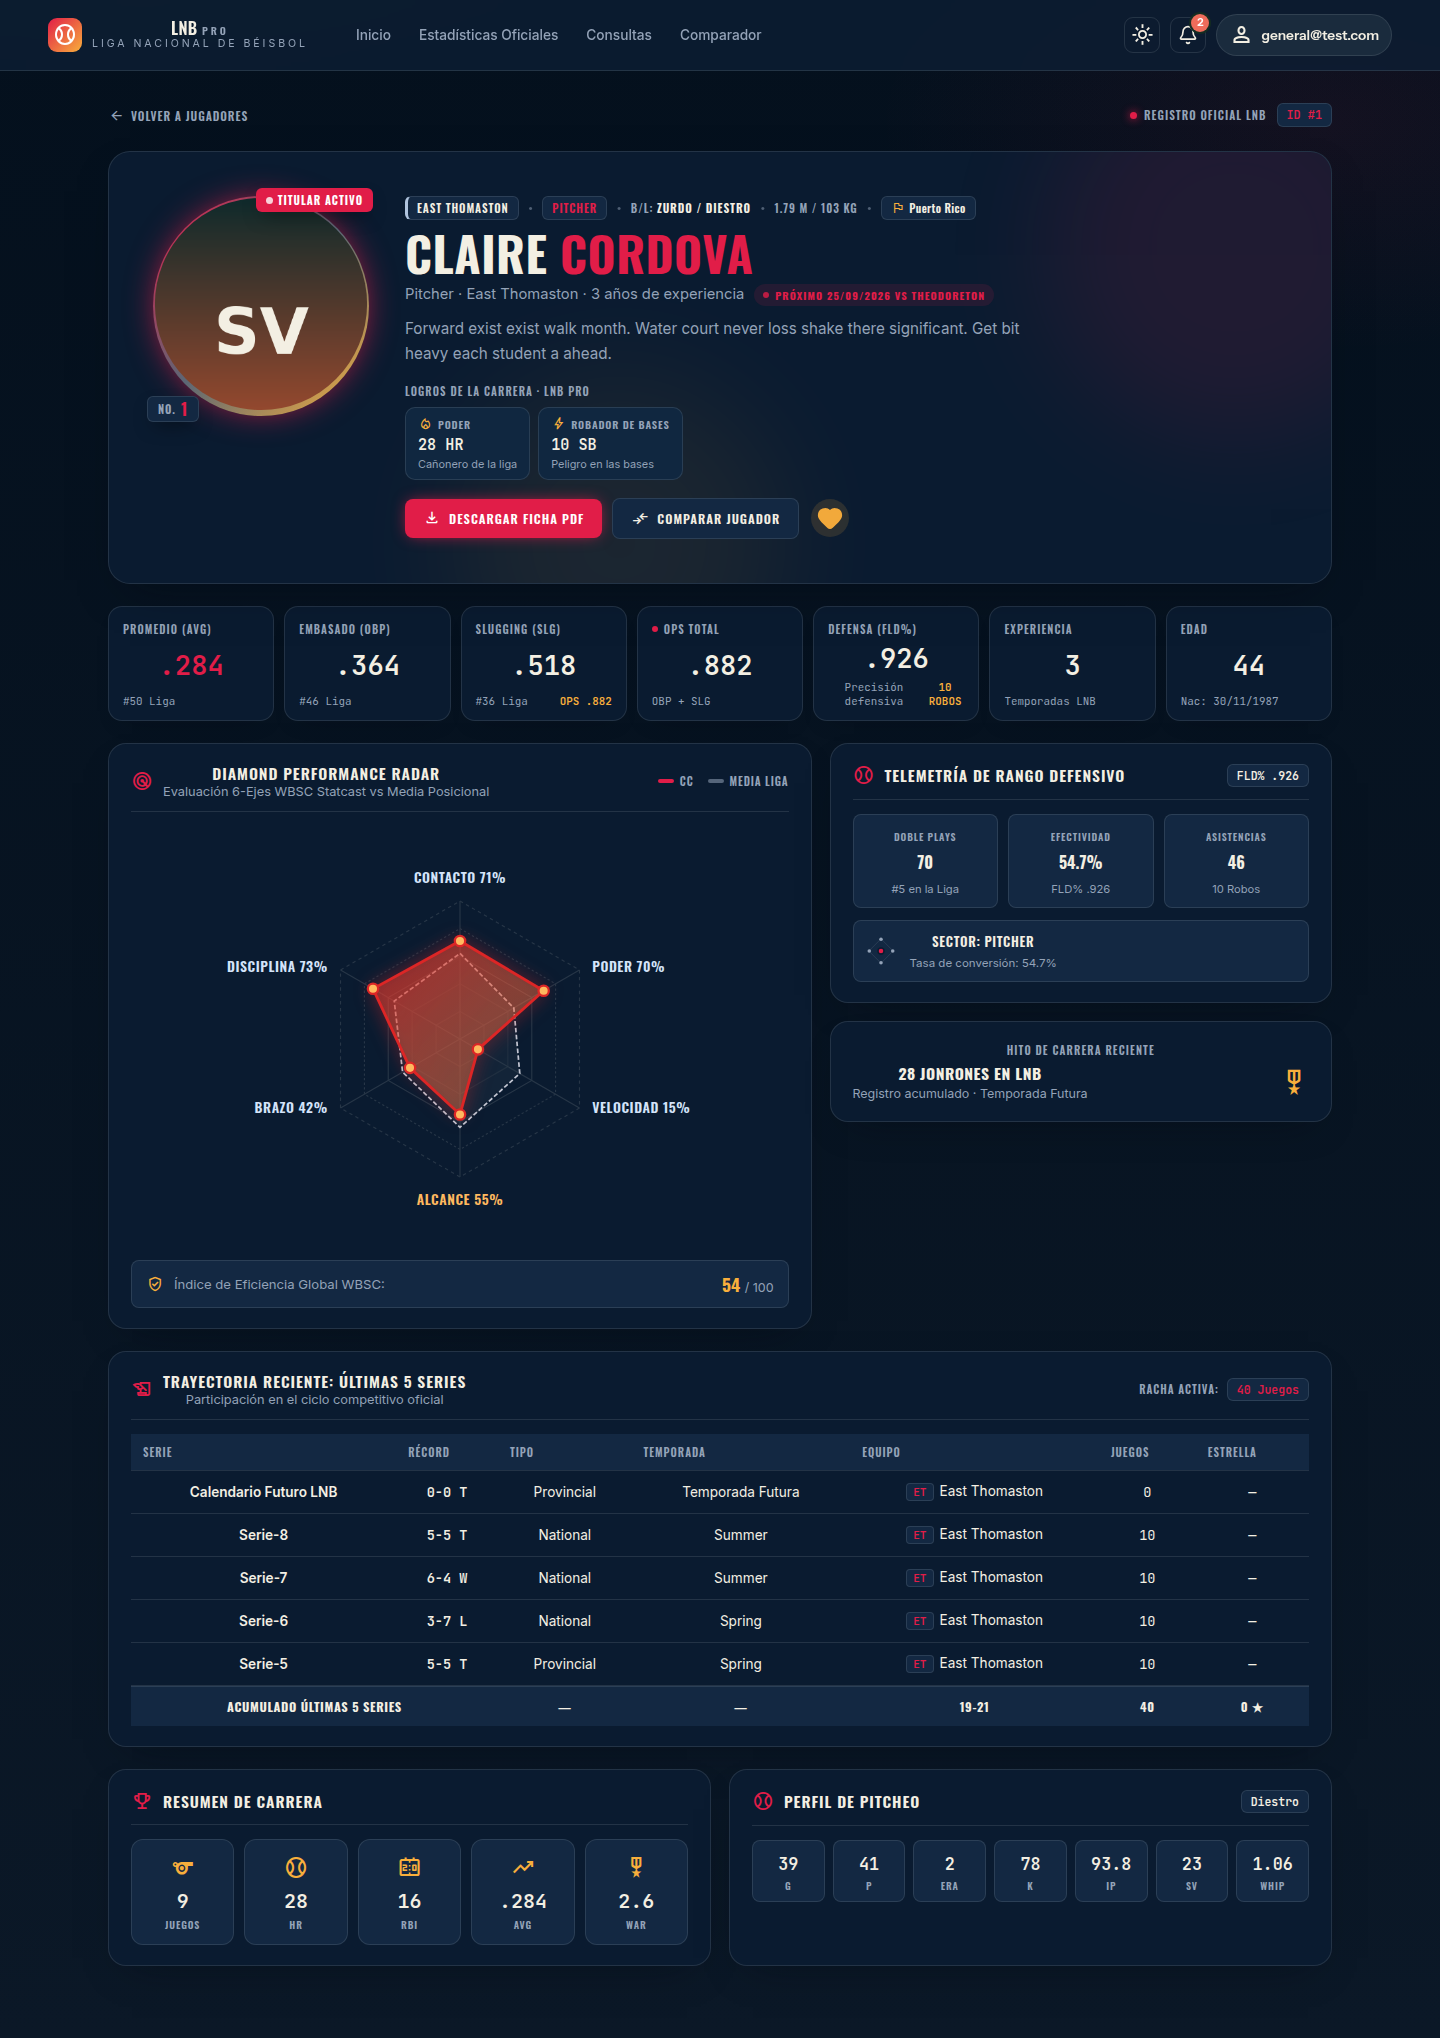
\includegraphics[width=0.7\textwidth]{img/img_14.png}
        \caption{Perfil de un jugador con el radar de rendimiento}
    \end{figure}

    \section*{Temas visuales}
    La aplicación ofrece dos temas: \textbf{oscuro} (por defecto) y \textbf{claro}, conmutables desde un
    botón en la cabecera. La elección se guarda en el navegador y se aplica en todas las páginas. La paleta
    está basada en los colores de un estadio (noche, césped, tiza, luces y clay) y cumple los criterios de
    contraste de accesibilidad WCAG AA.

    \begin{figure}[H]
        \centering
        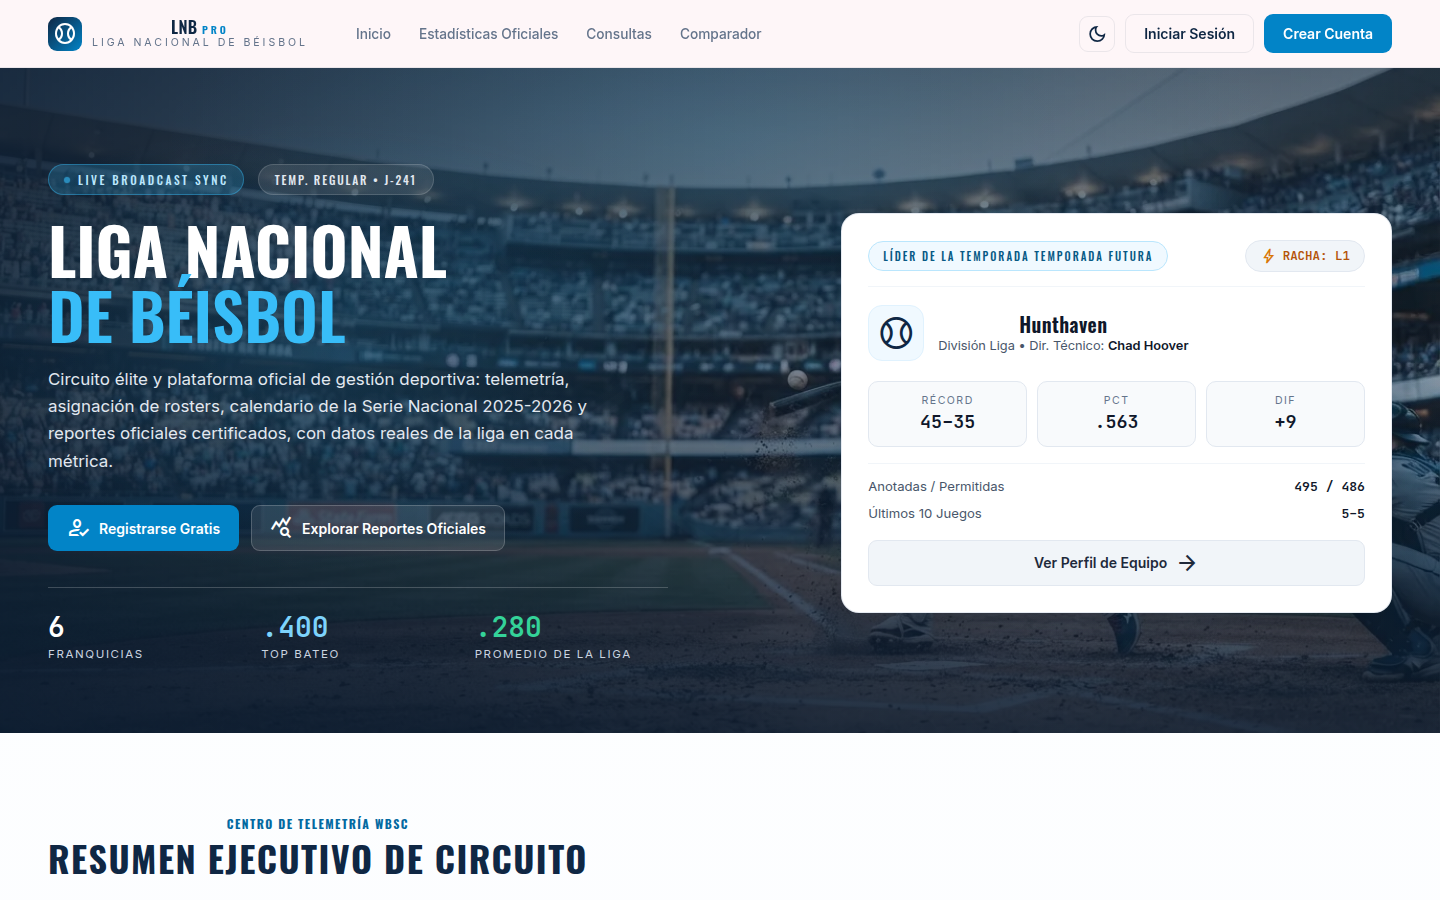
\includegraphics[width=0.62\textwidth]{img/img_15.png}
        \caption{Landing pública con el tema claro}
    \end{figure}

    \section*{Breve explicación de cada una de las salidas del sistema}
    \begin{itemize}
        \item \textbf{Exportación de reportes:} cada reporte oficial puede exportarse a \textbf{PDF} o
        \textbf{CSV} con la identidad visual de la LNB (marca, título y pie ``Afiliado Oficial WBSC'').
        Este botón está restringido a los usuarios con sesión iniciada; los invitados ven el candado.
        \item \textbf{Boleta técnica imprimible:} en el módulo de Estadísticas se puede descargar el
        \textbf{Boletín Técnico (PDF)} y \textbf{imprimir la boleta} con el corte completo de registros.
        \item \textbf{Ficha PDF del perfil de equipo:} el perfil de equipo permite descargar el roster
        oficial en PDF con la misma identidad corporativa (pie WBSC y paginación).
    \end{itemize}

\end{document}